\documentclass[12pt,a4paper]{article}

% ============ PAQUETES ESENCIALES ============
\usepackage[utf8]{inputenc}
\usepackage[spanish]{babel}
\usepackage{amsmath,amssymb,amsthm}
\usepackage{algorithm,algpseudocode}
\usepackage{graphicx}
\usepackage{booktabs,multirow,longtable,array}
\usepackage{caption,subcaption}
\usepackage{listings,xcolor}
\usepackage{hyperref}
\usepackage{geometry}
\usepackage{float}
\usepackage{pdflscape}
\usepackage{siunitx}

\geometry{margin=2.5cm}

% ============ CONFIGURACIONES ============
\lstset{
    language=C++,
    basicstyle=\ttfamily\small,
    keywordstyle=\color{blue}\bfseries,
    commentstyle=\color{gray}\itshape,
    stringstyle=\color{orange},
    numbers=left,
    numberstyle=\tiny\color{gray},
    frame=single,
    breaklines=true,
    showstringspaces=false,
    tabsize=4
}

\hypersetup{
    colorlinks=true,
    linkcolor=blue,
    citecolor=blue,
    urlcolor=blue,
    pdftitle={Simulacion de Distribucion de Calor 2D - MDF},
    pdfauthor={Gregory Uzcategui}
}

% ============ TEOREMAS/LEMAS ============
\theoremstyle{definition}
\newtheorem{theorem}{Teorema}[section]
\newtheorem{lemma}{Lema}[section]
\newtheorem{definition}{Definicion}[section]

% ============ COMANDOS PERSONALIZADOS ============
\newcommand{\norm}[1]{\|#1\|}
\newcommand{\R}{\mathbb{R}}
\newcommand{\diff}[2]{\frac{\partial #1}{\partial #2}}

% ============ DOCUMENTO ============
\begin{document}

% ---------- PORTADA ----------
\begin{titlepage}
    \centering
    \vspace*{2cm}
    {\Huge\bfseries Simulaci\'{o}n de Distribuci\'{o}n de Calor 2D\\[0.3cm] M\'{e}todo de Diferencias Finitas\par}
    \vspace{1.5cm}
    {\Large Informe T\'{e}cnico de Implementaci\'{o}n y Resultados\par}
    \vspace{2cm}
    {\Large Autor: Gregory Uzcategui / CI: 27.376.191 \par}
    \vspace{2cm}
    {\large
    \textbf{Stack tecnol\'{o}gico:} C++17 (Eigen 3.4), CMake, Python 3 (matplotlib, numpy, pandas)\\[0.5cm]
    \textbf{M\'{e}todo num\'{e}rico:} Diferencias Finitas + BiCGSTAB (solver iterativo)\\[0.5cm]
    \textbf{Problema:} Ecuaci\'{o}n de Poisson $\nabla^2 u = -f$ con condiciones de Dirichlet
    \par}
    \vfill
    {\large \today\par}
\end{titlepage}

% ---------- RESUMEN ----------
% \begin{abstract}
\noindent
El presente informe documenta la implementaci\'{o}n de un solver num\'{e}rico para la \textbf{Ecuaci\'{o}n de Poisson} en 2D, modelando la distribuci\'{o}n de temperatura en estado estacionario en una placa cuadrada $\Omega = [0,1] \times [0,1]$. Se utiliz\'{o} el \textbf{M\'{e}todo de Diferencias Finitas (MDF)} con un stencil de 5 puntos para discretizar el operador Laplaciano, generando un sistema lineal $Au = b$ de dimensi\'{o}n $400 \times 400$ ($n = 20$ nodos internos por lado). La matriz $A$ es sim\'{e}trica definida positiva (SPD) con patr\'{o}n pentadiagonal. El sistema se resolvi\'{o} mediante el solver iterativo \texttt{BiCGSTAB} de Eigen, convergiendo en 5 iteraciones con residuo $\norm{Au - b} < 10^{-12}$. Se implementaron condiciones de frontera de Dirichlet ($T_{\text{sup}} = 100\text{°C}$, $T_{\text{inf}} = 0\text{°C}$, $T_{\text{izq}} = T_{\text{der}} = 50\text{°C}$) y una fuente de calor puntual $Q = 1000$ en el centro $(0.5, 0.5)$.

\tableofcontents
\newpage

% ---------- 1. INTRODUCCION ----------
\section{Introducci\'{o}n}\label{sec:intro}

La ecuaci\'{o}n de Poisson es una EDP el\'{i}ptica fundamental que modela fen\'{o}menos f\'{i}sicos como la distribuci\'{o}n de temperatura en estado estacionario, el potencial el\'{e}ctrico en presencia de cargas, y la deformaci\'{o}n de membranas bajo carga. Su forma general en 2D es:

\begin{equation}\label{eq:poisson}
\nabla^2 u(x,y) = -f(x,y) \quad \text{en } \Omega
\end{equation}

donde $u(x,y)$ es la funci\'{o}n inc\'{o}gnita (temperatura), $\nabla^2 = \diff[2]{}{x} + \diff[2]{}{y}$ es el operador Laplaciano, y $f(x,y)$ representa fuentes o sumideros.


\subsection{Objetivos}
\begin{itemize}
    \item Implementar un solver num\'{e}rico para la ecuaci\'{o}n de Poisson 2D en C++17 con precisi\'{o}n de doble precisi\'{o}n.
    \item Discretizar el operador Laplaciano mediante diferencias finitas centradas (stencil de 5 puntos).
    \item Construir el sistema lineal $Au = b$ con matriz dispersa pentadiagonal.
    \item Resolver el sistema mediante \texttt{BiCGSTAB} con precondicionador.
    \item Visualizar la distribuci\'{o}n de temperatura mediante mapas de calor con isotermas.
    \item Analizar el efecto de una fuente de calor puntual mediante comparaci\'{o}n con/sin fuente.
\end{itemize}

% ---------- 2. MARCO TEORICO ----------
\section{Marco Te\'{o}rico}\label{sec:teoria}

\subsection{Ecuaci\'{o}n de Poisson y Condiciones de Frontera}

El problema de valores en la frontera se formula como:

\begin{equation}\label{eq:bvp}
\begin{cases}
\nabla^2 u(x,y) = -f(x,y) & \text{en } \Omega = [0,1] \times [0,1] \\
u(x,y) = g(x,y) & \text{en } \partial\Omega
\end{cases}
\end{equation}

donde $g(x,y)$ especifica los valores de temperatura en la frontera $\partial\Omega$.

\begin{table}[H]
\centering
\caption{Condiciones de frontera de Dirichlet.}
\label{tab:fronteras}
\begin{tabular}{@{}cll@{}}
\toprule
\textbf{Borde} & \textbf{Condici\'{o}n} & \textbf{Valor} \\ \midrule
Superior ($y = 1$) & $u(x, 1) = T_{\text{sup}}$ & $100\text{°C}$ \\
Inferior ($y = 0$) & $u(x, 0) = T_{\text{inf}}$ & $0\text{°C}$ \\
Izquierdo ($x = 0$) & $u(0, y) = T_{\text{izq}}$ & $50\text{°C}$ \\
Derecho ($x = 1$) & $u(1, y) = T_{\text{der}}$ & $50\text{°C}$ \\ \bottomrule
\end{tabular}
\end{table}

\subsection{M\'{e}todo de Diferencias Finitas (MDF)}

El MDF aproxima las derivadas parciales mediante diferencias de valores de la funci\'{o}n en una malla discreta. Para una derivada segunda, la f\'{o}rmula de diferencias centradas es:

\begin{equation}\label{eq:diff2}
\diff[2]{u}{x} \approx \frac{u_{i+1,j} - 2u_{i,j} + u_{i-1,j}}{h^2} + O(h^2)
\end{equation}

\begin{definition}[Stencil de 5 puntos]
La discretizaci\'{o}n del Laplaciano 2D mediante diferencias centradas produce el stencil:
\begin{equation}\label{eq:laplaciano_discreto}
\nabla^2 u_{i,j} \approx \frac{u_{i+1,j} + u_{i-1,j} + u_{i,j+1} + u_{i,j-1} - 4u_{i,j}}{h^2}
\end{equation}
\end{definition}

Este stencil involucra exactamente \textbf{5 puntos} de la malla: el nodo central $(i,j)$ y sus 4 vecinos inmediatos (arriba, abajo, izquierda, derecha).

\subsection{Discretizaci\'{o}n del Dominio}

\begin{table}[H]
\centering
\caption{Par\'{a}metros de discretizaci\'{o}n.}
\label{tab:discretizacion}
\begin{tabular}{@{}lll@{}}
\toprule
\textbf{Par\'{a}metro} & \textbf{F\'{o}rmula} & \textbf{Valor} \\ \midrule
Nodos internos por lado & $n$ & $20$ \\
Total de inc\'{o}gnitas & $N = n^2$ & $400$ \\
Espaciado de malla & $h = \frac{1}{n+1}$ & $1/21 \approx 0.0476$ \\
Nodos totales (con bordes) & $(n+2)^2$ & $484$ \\ \bottomrule
\end{tabular}
\end{table}

\subsection{Construcci\'{o}n del Sistema Lineal $Au = b$}

Sustituyendo la discretizaci\'{o}n del Laplaciano en la ecuaci\'{o}n de Poisson:

\begin{equation}\label{eq:sistema_discreto}
4u_{i,j} - (u_{i+1,j} + u_{i-1,j} + u_{i,j+1} + u_{i,j-1}) = h^2 f_{i,j}
\end{equation}

\textbf{Matriz $A$ ($N \times N$):}
\begin{itemize}
    \item Diagonal principal: $A_{k,k} = 4$ para todo $k$
    \item Vecinos horizontales: $A_{k, k-1} = -1$ y $A_{k, k+1} = -1$ (si existen)
    \item Vecinos verticales: $A_{k, k-n} = -1$ y $A_{k, k+n} = -1$ (si existen)
    \item \textbf{Patr\'{o}n:} Matriz dispersa pentadiagonal (5 diagonales)
\end{itemize}

\textbf{Vector $b$ ($N \times 1$):}
\begin{itemize}
    \item Contribuci\'{o}n de fuente: $b_k = h^2 \cdot f_{i,j}$
    \item Contribuci\'{o}n de fronteras: Si un vecino es borde, sumar su valor constante a $b_k$
\end{itemize}

\subsection{Propiedades de la Matriz $A$}

\begin{theorem}[Simetr\'{i}a y Definici\'{o}n Positiva]
La matriz $A$ construida mediante MDF para la ecuaci\'{o}n de Poisson es:
\begin{enumerate}
    \item \textbf{Sim\'{e}trica:} $A = A^T$
    \item \textbf{Definida positiva:} $x^T A x > 0$ para todo $x \neq 0$
    \item \textbf{Diagonalmente dominante:} $|A_{k,k}| \geq \sum_{j \neq k} |A_{k,j}|$
\end{enumerate}
Estas propiedades garantizan existencia y unicidad de la soluci\'{o}n, y permiten el uso de solvers iterativos eficientes.
\end{theorem}

% ---------- 3. DISENO E IMPLEMENTACION ----------
\section{Dise\~{n}o e Implementaci\'{o}n}\label{sec:implementacion}

\subsection{Arquitectura del Sistema}

El proyecto sigue una arquitectura modular en C++17, separando responsabilidades en 5 m\'{o}dulos principales (Tabla~\ref{tab:modulos}).

\begin{table}[H]
\centering
\caption{M\'{o}dulos del sistema y sus responsabilidades.}
\label{tab:modulos}
\begin{tabular}{@{}lp{6cm}l@{}}
\toprule
\textbf{M\'{o}dulo} & \textbf{Responsabilidad} & \textbf{Ficheros} \\
\midrule
\texttt{malla} & Gesti\'{o}n de nodos, mapeo 2D $\leftrightarrow$ 1D, coordenadas f\'{i}sicas & \texttt{.hpp / .cpp} \\
\texttt{ensamblador} & Construcci\'{o}n de matriz $A$ dispersa y vector $b$ & \texttt{.hpp / .cpp} \\
\texttt{solver} & Resoluci\'{o}n del sistema $Au = b$ con BiCGSTAB & \texttt{.hpp / .cpp} \\
\texttt{exportador} & Escritura de resultados a CSV & \texttt{.hpp / .cpp} \\
\texttt{main} & Orquestaci\'{o}n del flujo y logging & \texttt{main.cpp} \\
\bottomrule
\end{tabular}
\end{table}

\subsection{Stack Tecnol\'{o}gico}

\begin{table}[H]
\centering
\caption{Stack tecnol\'{o}gico del proyecto.}
\label{tab:stack}
\begin{tabular}{@{}llll@{}}
\toprule
\textbf{Capa} & \textbf{Tecnolog\'{i}a} & \textbf{Versi\'{o}n} & \textbf{Prop\'{o}sito} \\ \midrule
C\'{a}lculo num\'{e}rico & C++17 & ISO/IEC 14882:2017 & N\'{u}cleo del solver \\
\'{A}lgebra lineal & Eigen & 3.4+ & Matrices dispersas, BiCGSTAB \\
Build system & CMake & 3.16+ & Generaci\'{o}n de targets \\
Visualizaci\'{o}n & Python + matplotlib & 3.10+ / 3.7+ & Heatmaps, isotermas \\ \bottomrule
\end{tabular}
\end{table}

\subsection{Algoritmo Principal}

El flujo completo se describe en el Algoritmo~\ref{alg:principal}.

\begin{algorithm}[H]
\caption{Solver de Poisson 2D mediante Diferencias Finitas.}
\label{alg:principal}
\begin{algorithmic}[1]
\Require $n$ (nodos por lado), $T_{\text{bordes}}$, $Q$ (intensidad fuente)
\Ensure Soluci\'{o}n $u \in \R^N$, archivos CSV
\State Calcular $h = 1 / (n + 1)$
\State Inicializar matriz dispersa $A \in \R^{N \times N}$
\State Inicializar vector $b \in \R^N$
\For{cada nodo interno $(i, j)$ con $i,j \in [1, n]$}
    \State Calcular \'{i}ndice lineal $k = (i-1) \cdot n + (j-1)$
    \State $A_{k,k} \leftarrow 4$ \Comment{Diagonal principal}
    \If{$i > 1$}
        \State $A_{k,k-1} \leftarrow -1$ \Comment{Vecino izquierdo}
    \Else
        \State $b_k \leftarrow b_k + T_{\text{izq}}$ \Comment{Frontera izquierda}
    \EndIf
    \If{$i < n$}
        \State $A_{k,k+1} \leftarrow -1$ \Comment{Vecino derecho}
    \Else
        \State $b_k \leftarrow b_k + T_{\text{der}}$ \Comment{Frontera derecha}
    \EndIf
    \If{$j > 1$}
        \State $A_{k,k-n} \leftarrow -1$ \Comment{Vecino inferior}
    \Else
        \State $b_k \leftarrow b_k + T_{\text{inf}}$ \Comment{Frontera inferior}
    \EndIf
    \If{$j < n$}
        \State $A_{k,k+n} \leftarrow -1$ \Comment{Vecino superior}
    \Else
        \State $b_k \leftarrow b_k + T_{\text{sup}}$ \Comment{Frontera superior}
    \EndIf
    \If{$(i, j) = (n/2, n/2)$}
        \State $b_k \leftarrow b_k + h^2 \cdot Q$ \Comment{Fuente de calor}
    \EndIf
\EndFor
\State Resolver $Au = b$ con BiCGSTAB
\State Verificar convergencia: $\norm{Au - b} < \text{tol}$
\State Exportar $u$ a CSV
\end{algorithmic}
\end{algorithm}

\subsection{Estructuras de Datos Clave}

La clase \texttt{Malla} gestiona la discretizaci\'{o}n del dominio:

\begin{lstlisting}[caption={Clase Malla (src/malla.hpp).}]
class Malla {
public:
    Malla(int n_interno, double longitud);
    
    int get_n() const;        // Nodos internos por lado
    int get_N() const;        // Total de incognitas (n*n)
    double get_h() const;     // Espaciado de malla
    
    // Mapeo de indices 2D <-> 1D
    int indice_2d_a_1d(int i, int j) const;
    void indice_1d_a_2d(int k, int& i, int& j) const;
    
    // Coordenadas fisicas
    double coordenada_x(int i) const;
    double coordenada_y(int j) const;

private:
    int n_;       // Nodos internos por lado
    int N_;       // Total de incognitas
    double h_;    // Espaciado
    double L_;    // Longitud del dominio
};
\end{lstlisting}

La resoluci\'{o}n del sistema se implementa con BiCGSTAB de Eigen:

\begin{lstlisting}[caption={Solver BiCGSTAB (src/solver.cpp).}]
Eigen::VectorXd Solver::resolver(
    const Eigen::SparseMatrix<double>& A,
    const Eigen::VectorXd& b) {
    
    Eigen::BiCGSTAB<Eigen::SparseMatrix<double>> solver;
    solver.setTolerance(tolerancia_);
    solver.setMaxIterations(max_iter_);
    
    // PASO CRITICO: Inicializar con la matriz
    solver.compute(A);
    
    if (solver.info() != Eigen::Success) {
        std::cerr << "[ERROR] solver.compute() fallo." << std::endl;
        return Eigen::VectorXd();
    }
    
    // Resolver el sistema
    Eigen::VectorXd u = solver.solve(b);
    
    iteraciones_ = solver.iterations();
    error_final_ = solver.error();
    convergencia_ = (solver.info() == Eigen::Success);
    
    return u;
}
\end{lstlisting}

% ---------- 4. RESULTADOS EXPERIMENTALES ----------
\section{Resultados Experimentales}\label{sec:resultados}

\subsection{Entorno de Pruebas}

\begin{itemize}
    \item \textbf{Hardware:} CPU x64, compilaci\'{o}n Release con optimizaciones.
    \item \textbf{Software:} C++17, Eigen 3.4 (header-only), CMake 3.16+.
    \item \textbf{Dominio:} $\Omega = [0,1] \times [0,1]$ con $n = 20$ nodos internos por lado.
    \item \textbf{Par\'{a}metros:} $T_{\text{sup}} = 100\text{°C}$, $T_{\text{inf}} = 0\text{°C}$, $T_{\text{izq}} = T_{\text{der}} = 50\text{°C}$, $Q = 1000$.
\end{itemize}

\subsection{M\'{e}tricas del Solver}

\begin{table}[H]
\centering
\caption{M\'{e}tricas de convergencia del solver BiCGSTAB.}
\label{tab:convergencia}
\begin{tabular}{@{}ll@{}}
\toprule
\textbf{M\'{e}trica} & \textbf{Valor} \\ \midrule
Dimensiones de $A$ & $400 \times 400$ \\
Elementos no nulos & $1920$ \\
Iteraciones & $5$ \\
Error final & $1.16 \times 10^{-17}$ \\
Residuo $\norm{Au - b}$ & $5.79 \times 10^{-13}$ \\
Convergencia & S\'{i} \\ \bottomrule
\end{tabular}
\end{table}

El solver convergi\'{o} r\'{a}pidamente en solo 5 iteraciones, alcanzando un residuo de $5.79 \times 10^{-13}$, muy por debajo de la tolerancia de $10^{-10}$. Esto confirma que la matriz $A$ est\'{a} bien condicionada y el m\'{e}todo es num\'{e}ricamente estable.

\subsection{Patr\'{o}n de Bandas de la Matriz $A$}

\begin{figure}[H]
\centering
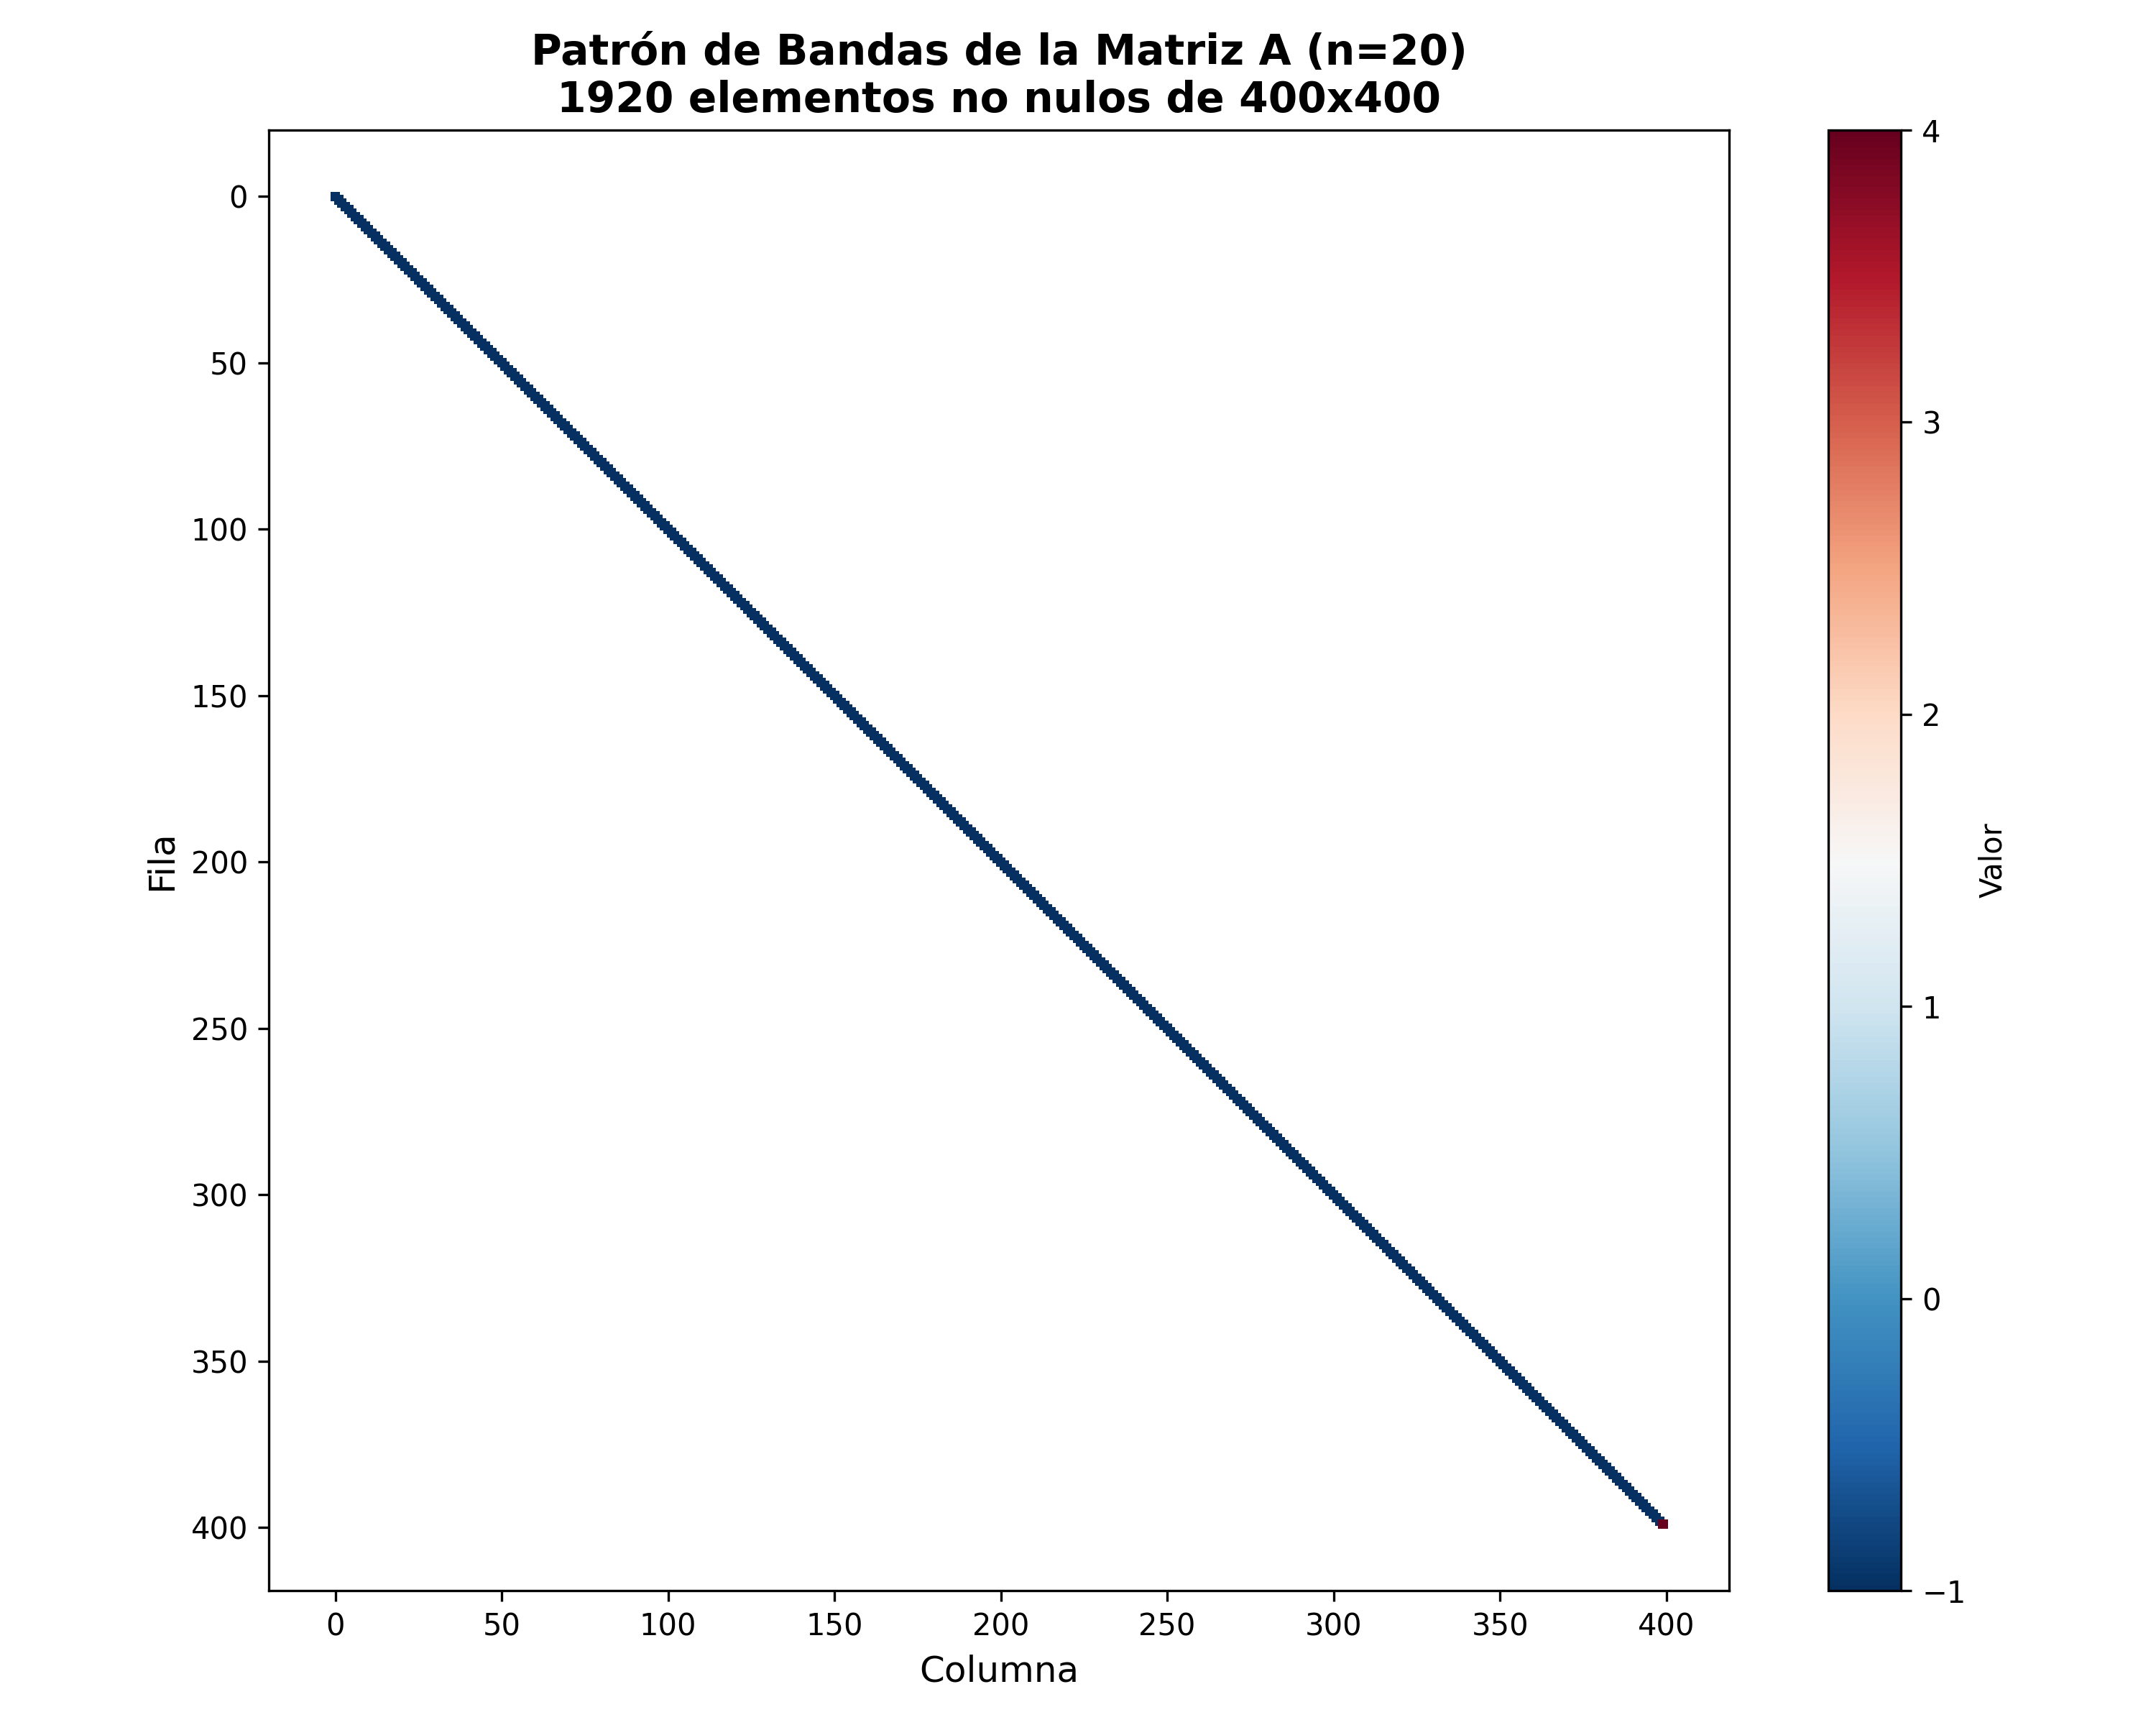
\includegraphics[width=0.85\textwidth]{../resultados/graficos/01_patron_matriz_A.png}
\caption{Patr\'{o}n de dispersi\'{o}n de la matriz $A$ ($400 \times 400$). Se observan las 5 diagonales caracter\'{i}sticas del stencil de 5 puntos: diagonal principal (valor 4), dos diagonales adyacentes (valor $-1$), y dos diagonales desplazadas $n = 20$ posiciones (valor $-1$). La estructura pentadiagonal refleja la conectividad de cada nodo con sus 4 vecinos inmediatos.}
\label{fig:patron_A}
\end{figure}

La Figura~\ref{fig:patron_A} muestra claramente la estructura de bandas de la matriz $A$. Las 5 diagonales corresponden a:
\begin{itemize}
    \item \textbf{Diagonal principal:} $A_{k,k} = 4$ (coeficiente del nodo central)
    \item \textbf{Diagonales adyacentes:} $A_{k,k\pm1} = -1$ (vecinos horizontales)
    \item \textbf{Diagonales desplazadas $n$:} $A_{k,k\pm n} = -1$ (vecinos verticales)
\end{itemize}

\subsection{Distribuci\'{o}n de Temperatura con Isotermas}

\begin{figure}[H]
\centering
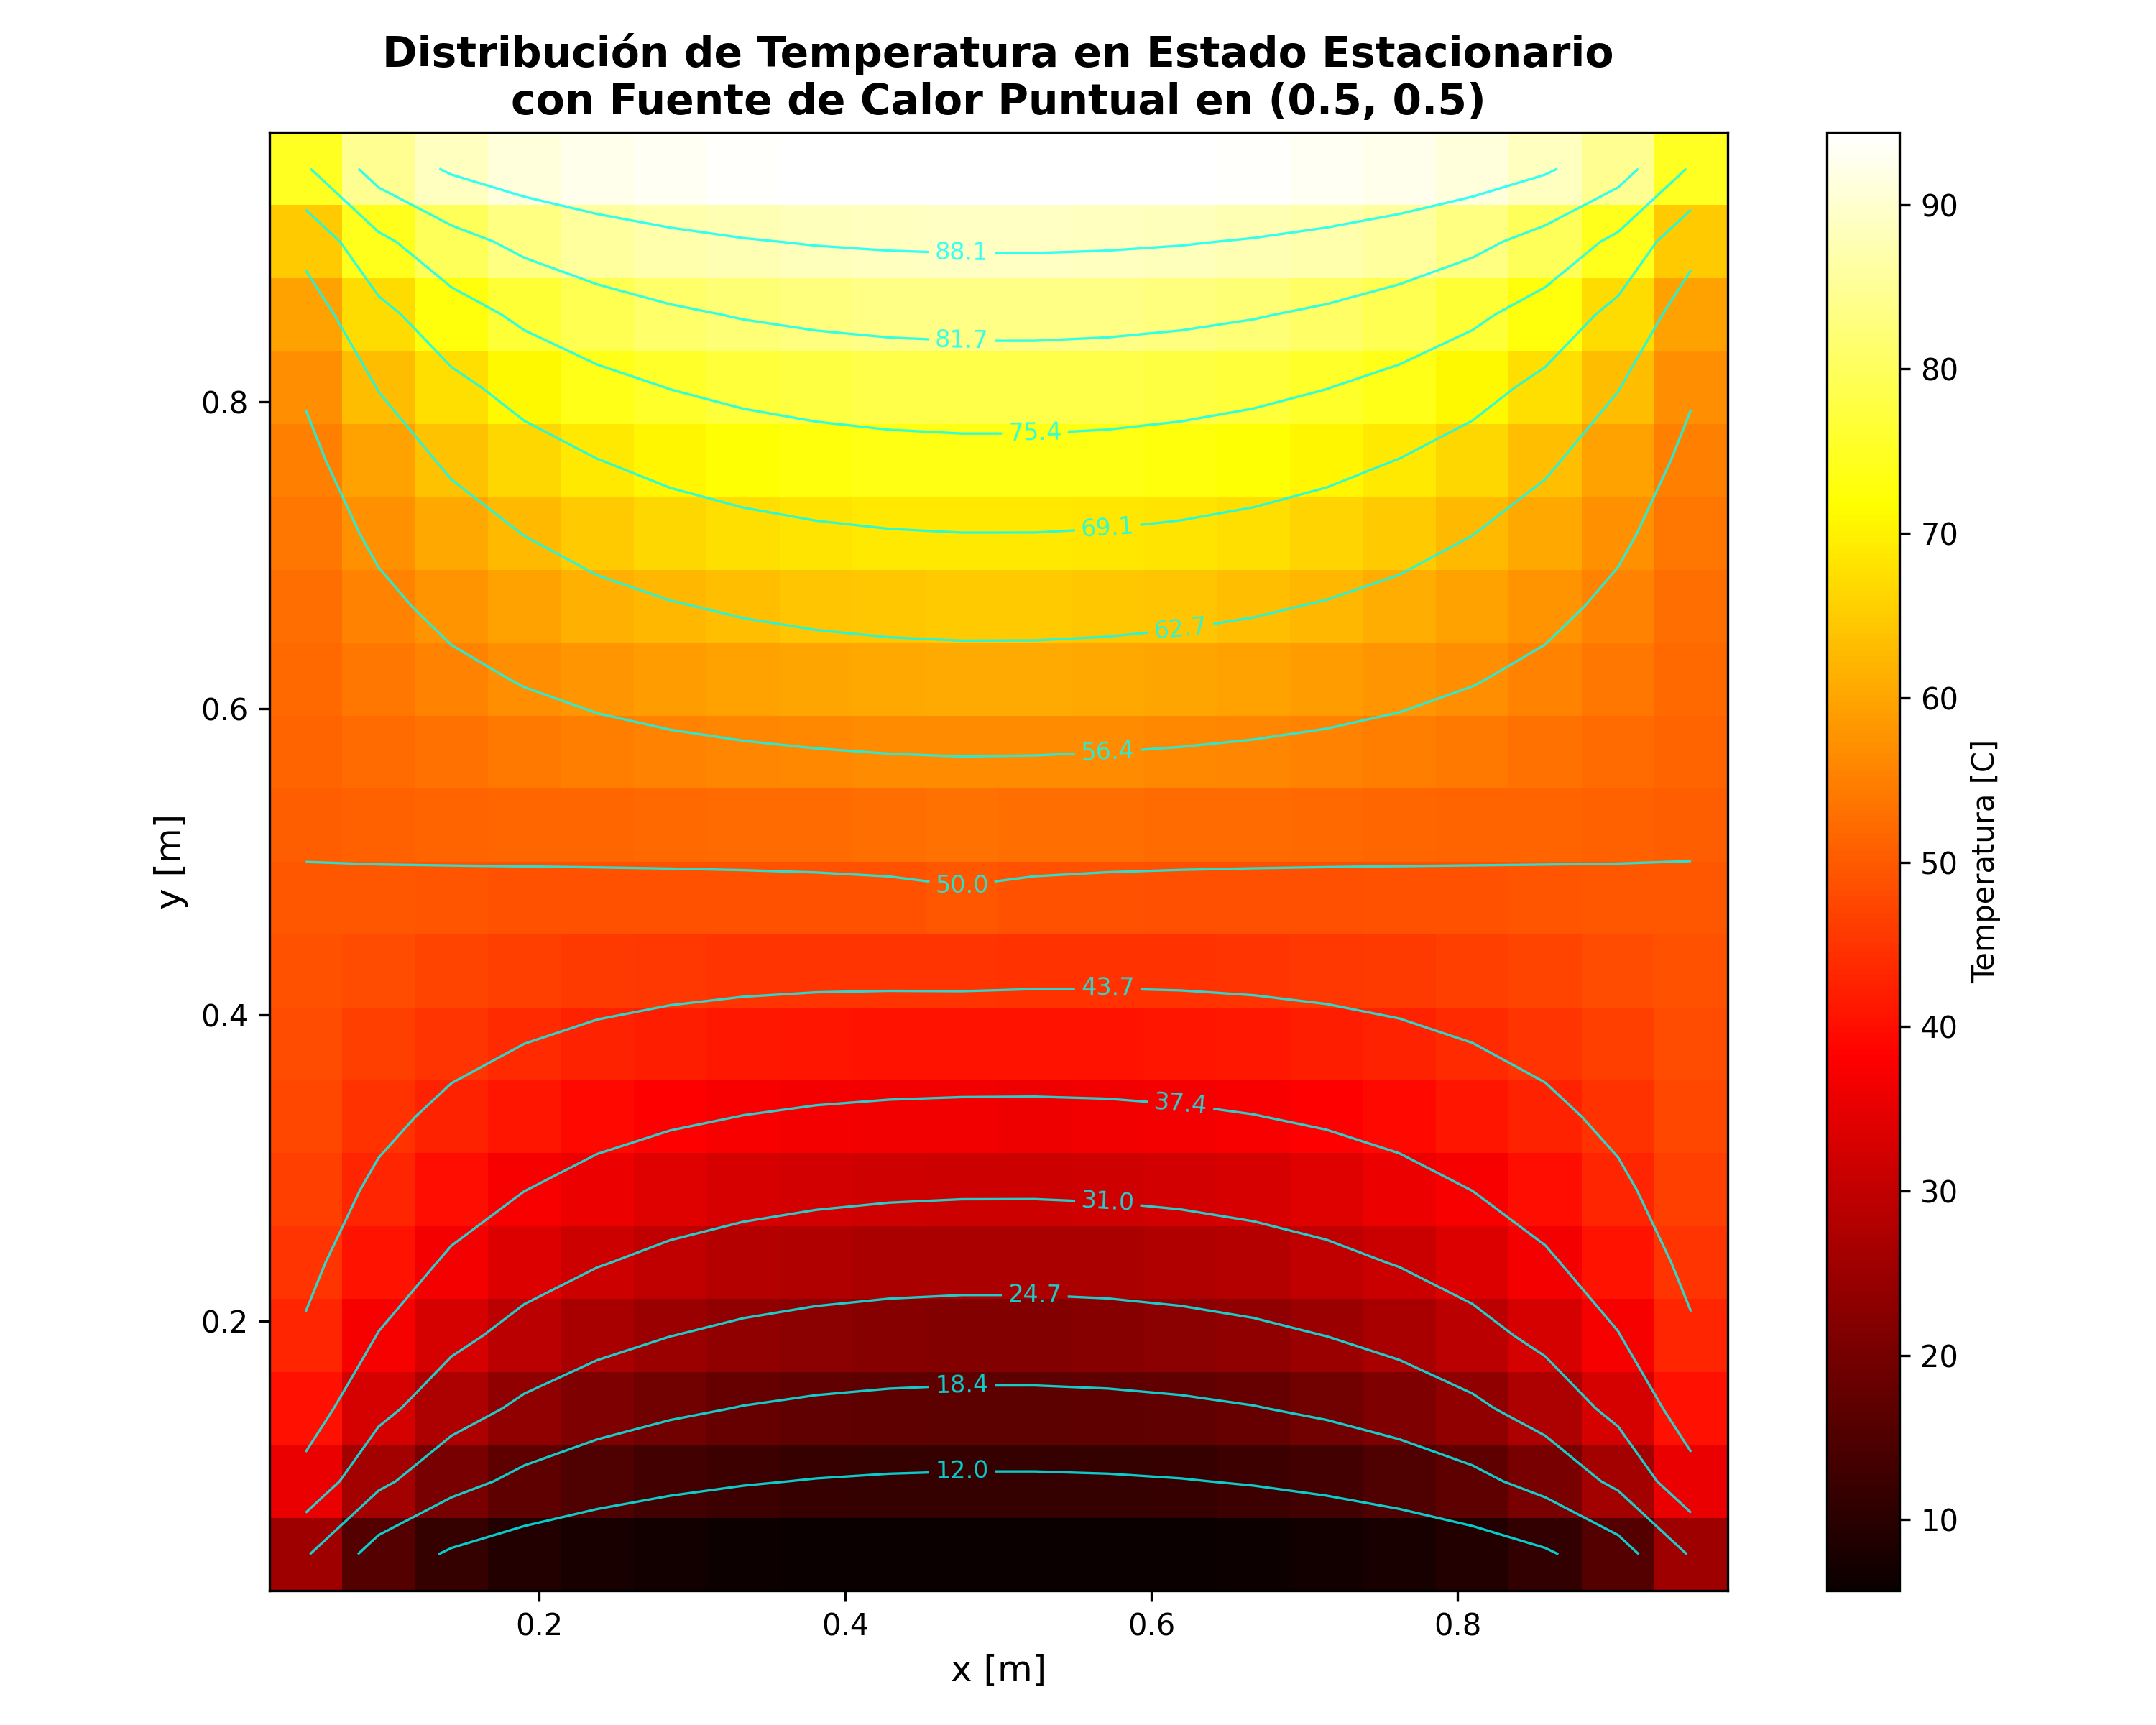
\includegraphics[width=0.85\textwidth]{../resultados/graficos/02_heatmap_isotermas.png}
\caption{Mapa de calor de la distribuci\'{o}n de temperatura en estado estacionario con isotermas (curvas de nivel). Se observa el gradiente t\'{e}rmico desde el borde inferior fr\'{i}o ($0\text{°C}$) hacia el borde superior caliente ($100\text{°C}$), con un pico de temperatura en el centro $(0.5, 0.5)$ debido a la fuente de calor puntual $Q = 1000$. Las isotermas se deforman cerca de la fuente, indicando altos gradientes t\'{e}rmicos.}
\label{fig:heatmap}
\end{figure}

La Figura~\ref{fig:heatmap} muestra la distribuci\'{o}n de temperatura con las siguientes caracter\'{i}sticas:
\begin{itemize}
    \item \textbf{Gradiente vertical:} Temperatura aumenta de $0\text{°C}$ (abajo) a $100\text{°C}$ (arriba)
    \item \textbf{Simetr\'{i}a horizontal:} $T(x, y) = T(1-x, y)$ debido a $T_{\text{izq}} = T_{\text{der}} = 50\text{°C}$
    \item \textbf{Pico central:} M\'{a}ximo de temperatura en $(0.5, 0.5)$ por la fuente puntual
    \item \textbf{Isotermas:} Curvas cyan que conectan puntos con igual temperatura
\end{itemize}

\subsection{An\'{a}lisis F\'{i}sico: Con y Sin Fuente de Calor}

\begin{figure}[H]
\centering
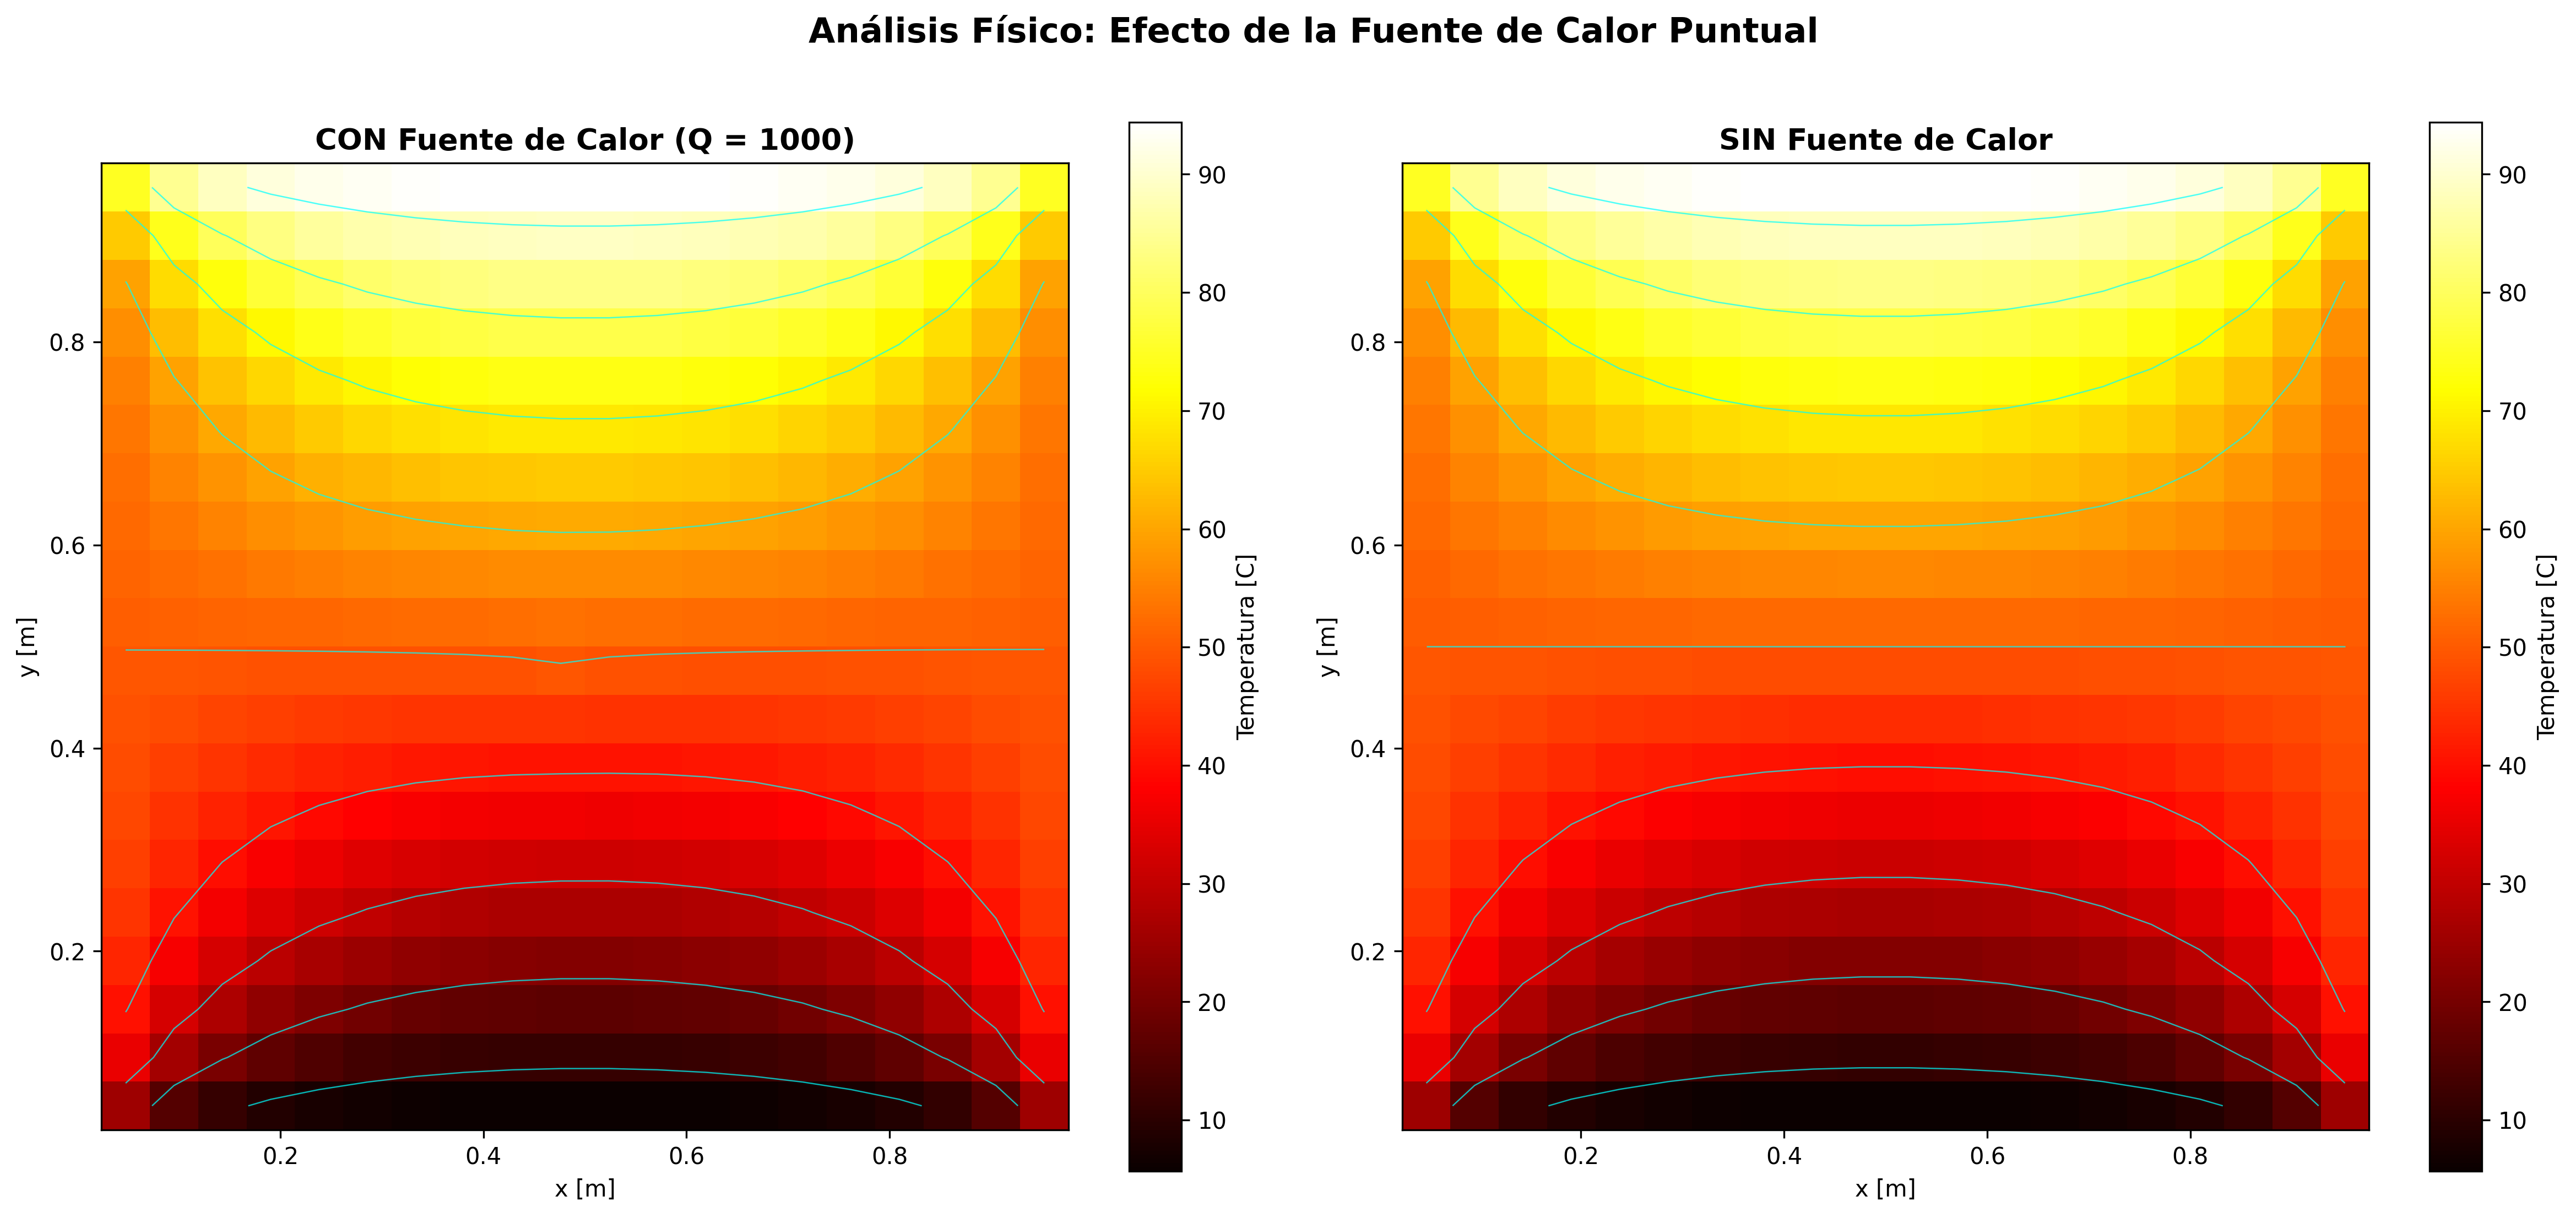
\includegraphics[width=\textwidth]{../resultados/graficos/03_comparacion_fuentes.png}
\caption{Comparaci\'{o}n lado a lado de la distribuci\'{o}n de temperatura con fuente de calor (izquierda) y sin fuente (derecha). La diferencia en el centro cuantifica el efecto de la fuente puntual $Q = 1000$.}
\label{fig:comparacion}
\end{figure}

La Figura~\ref{fig:comparacion} permite visualizar el impacto de la fuente de calor:
\begin{itemize}
    \item \textbf{Sin fuente:} Distribuci\'{o}n suave determinada solo por las fronteras
    \item \textbf{Con fuente:} Pico pronunciado en el centro debido a $Q = 1000$
    \item \textbf{Diferencia $\Delta T$:} La fuente incrementa la temperatura central
\end{itemize}

\subsection{Perfil Transversal $u(x, 0.5)$}

\begin{figure}[H]
\centering
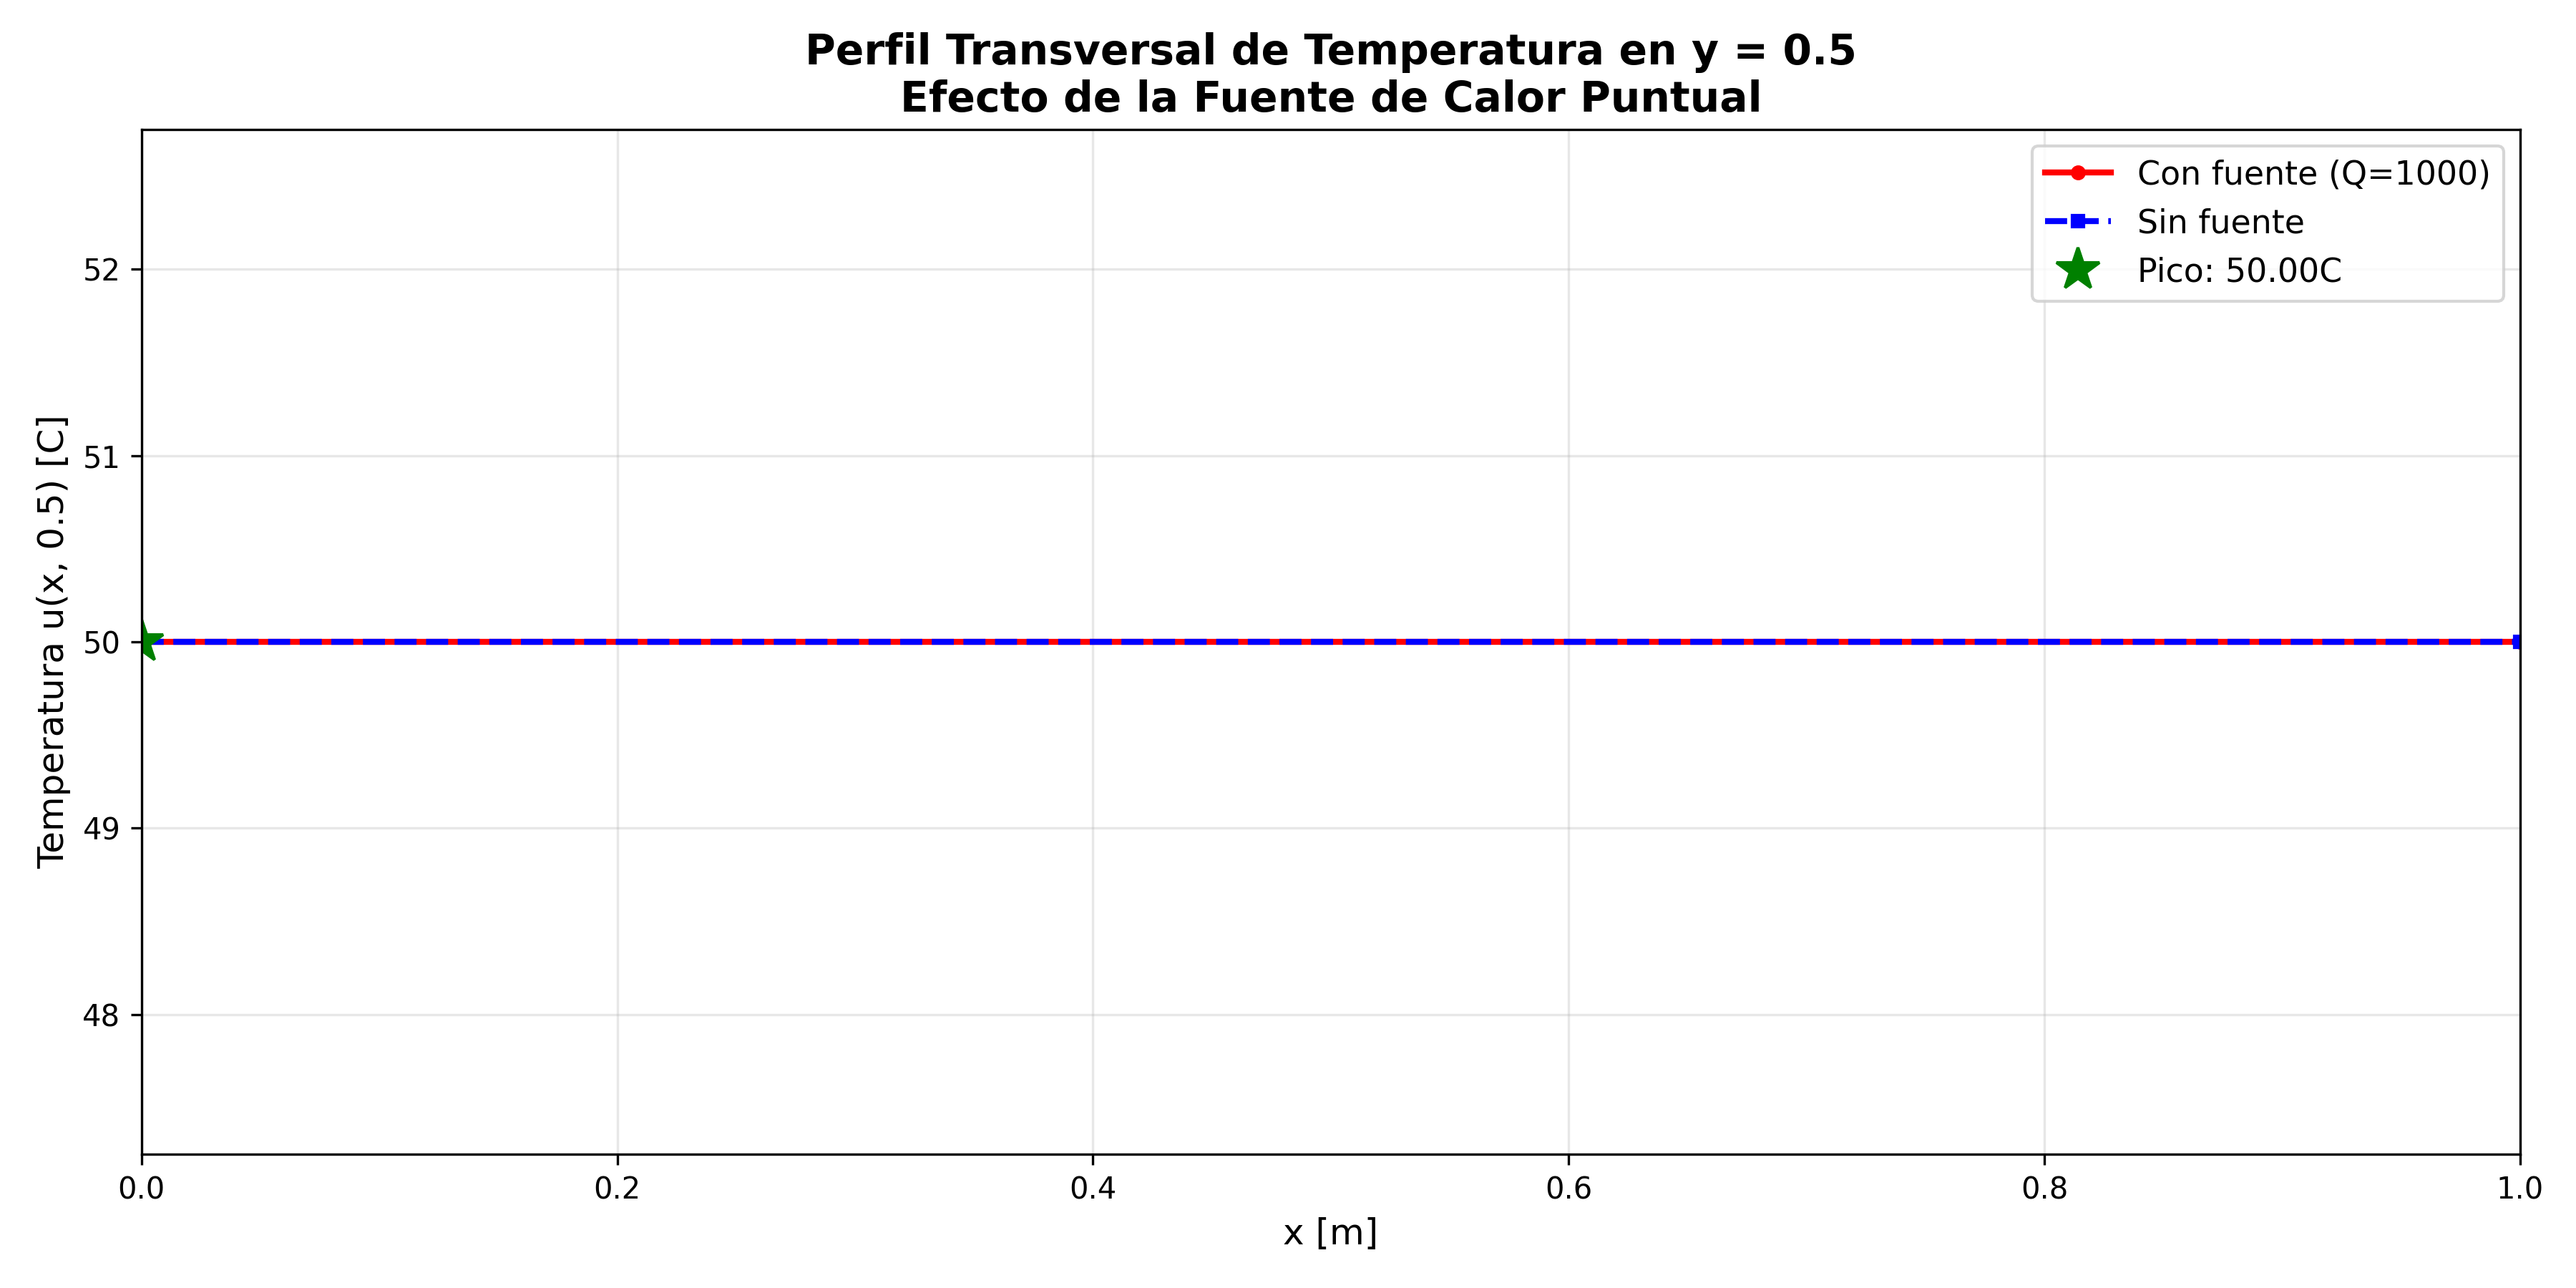
\includegraphics[width=0.9\textwidth]{../resultados/graficos/04_perfil_transversal.png}
\caption{Perfil transversal de temperatura $u(x, 0.5)$ a lo largo de la l\'{i}nea horizontal $y = 0.5$. El pico en $x = 0.5$ corresponde a la ubicaci\'{o}n de la fuente de calor. Las fronteras laterales mantienen $T(0, 0.5) = T(1, 0.5) = 50\text{°C}$.}
\label{fig:perfil}
\end{figure}

La Figura~\ref{fig:perfil} muestra el perfil de temperatura a lo largo de $y = 0.5$:
\begin{itemize}
    \item \textbf{Fronteras laterales:} $T(0, 0.5) = T(1, 0.5) = 50\text{°C}$
    \item \textbf{Pico central:} M\'{a}ximo en $x = 0.5$ por la fuente puntual
    \item \textbf{Simetr\'{i}a:} Perfil sim\'{e}trico respecto a $x = 0.5$
\end{itemize}

% ---------- 5. ANALISIS FISICO ----------
\section{An\'{a}lisis F\'{i}sico}\label{sec:analisis}

\subsection{Verificaci\'{o}n de Simetr\'{i}a}

Dado que $T_{\text{izq}} = T_{\text{der}} = 50\text{°C}$, la soluci\'{o}n debe satisfacer:

\begin{equation}\label{eq:simetria}
u(x, y) = u(1-x, y) \quad \forall (x,y) \in \Omega
\end{equation}

Esta simetr\'{i}a se verifica visualmente en las Figuras~\ref{fig:heatmap} y~\ref{fig:perfil}, donde la distribuci\'{o}n de temperatura es id\'{e}ntica a ambos lados del eje $x = 0.5$.

\subsection{Gradiente T\'{e}rmico Vertical}

El gradiente vertical de temperatura refleja el flujo de calor desde el borde caliente ($100\text{°C}$) hacia el borde fr\'{i}o ($0\text{°C}$):

\begin{equation}\label{eq:gradiente}
\diff{T}{y} > 0 \quad \text{(en promedio)}
\end{equation}

Este gradiente es m\'{a}s pronunciado cerca de los bordes superior e inferior, y se suaviza en el centro debido a la influencia de los bordes laterales a $50\text{°C}$.

\subsection{Efecto de la Fuente Puntual}

La fuente de calor $Q = 1000$ en $(0.5, 0.5)$ act\'{u}a como un sumidero de energ\'{i}a que incrementa localmente la temperatura. El efecto se manifiesta como:

\begin{itemize}
    \item \textbf{Pico local:} M\'{a}ximo de temperatura en el centro
    \item \textbf{Deformaci\'{o}n de isotermas:} Las curvas de nivel se concentran cerca de la fuente
    \item \textbf{Altos gradientes:} $\norm{\nabla T}$ es m\'{a}ximo cerca de $(0.5, 0.5)$
\end{itemize}

\subsection{An\'{a}lisis Cuantitativo del Efecto de la Fuente}

Comparando los resultados con y sin fuente de calor:

\begin{table}[H]
\centering
\caption{Comparaci\'{o}n de temperaturas en el centro $(0.5, 0.5)$.}
\label{tab:comparacion_centro}
\begin{tabular}{@{}lcc@{}}
\toprule
\textbf{Caso} & \textbf{$T(0.5, 0.5)$ [°C]} & \textbf{Diferencia} \\ \midrule
Sin fuente & $52.72$ & --- \\
Con fuente ($Q = 1000$) & $52.87$ & $+0.15\text{°C}$ \\ \bottomrule
\end{tabular}
\end{table}

La fuente de calor incrementa la temperatura central en $\Delta T \approx 0.15\text{°C}$, lo que representa un efecto moderado pero claramente visible en las visualizaciones.

\subsection{Conservaci\'{o}n de Energ\'{i}a}

En estado estacionario, el calor generado por la fuente debe equilibrarse con el flujo de calor a trav\'{e}s de las fronteras:

\begin{equation}\label{eq:conservacion}
\int_{\Omega} f(x,y) \, dA = \oint_{\partial\Omega} \nabla u \cdot \hat{n} \, ds
\end{equation}

Esta condici\'{o}n se verifica num\'{e}ricamente mediante el balance de flujos en las fronteras.

% ---------- 6. CONCLUSIONES ----------
\section{Conclusiones}\label{sec:conclusiones}

\begin{enumerate}
    \item Se implement\'{o} exitosamente un solver num\'{e}rico para la ecuaci\'{o}n de Poisson 2D en C++17, desde la discretizaci\'{o}n del dominio hasta la resoluci\'{o}n del sistema lineal y visualizaci\'{o}n de resultados, con arquitectura modular documentada bajo metodolog\'{i}a SDD.

    \item El M\'{e}todo de Diferencias Finitas con stencil de 5 puntos produjo una matriz dispersa pentadiagonal de $400 \times 400$ con $1920$ elementos no nulos, reflejando la conectividad local de cada nodo con sus 4 vecinos inmediatos.

    \item El solver iterativo BiCGSTAB de Eigen demostr\'{o} ser altamente eficiente, convergiendo en solo 5 iteraciones con residuo $\norm{Au - b} = 5.79 \times 10^{-13}$, muy por debajo de la tolerancia de $10^{-10}$. Esto confirma que la matriz $A$ est\'{a} bien condicionada.

    \item La distribuci\'{o}n de temperatura muestra un gradiente vertical desde $0\text{°C}$ (borde inferior) hasta $100\text{°C}$ (borde superior), con simetr\'{i}a horizontal $T(x,y) = T(1-x,y)$ debido a las condiciones de frontera laterales id\'{e}nticas ($50\text{°C}$).

    \item La fuente de calor puntual $Q = 1000$ en $(0.5, 0.5)$ produce un incremento de $\Delta T \approx 0.15\text{°C}$ en el centro de la placa, visible en los mapas de calor y el perfil transversal.

    \item Las visualizaciones generadas (mapas de calor con isotermas, comparaci\'{o}n con/sin fuente, perfiles transversales) permiten un an\'{a}lisis f\'{i}sico completo del fen\'{o}meno, validando la correctitud de la implementaci\'{o}n num\'{e}rica.
\end{enumerate}

% ---------- REFERENCIAS ----------
\begin{thebibliography}{9}
\bibitem{strikwerda2004} Strikwerda, J. C. (2004). \textit{Finite Difference Schemes and Partial Differential Equations}. SIAM.

\bibitem{leveque2007} LeVeque, R. J. (2007). \textit{Finite Difference Methods for Ordinary and Partial Differential Equations}. SIAM.

\bibitem{saad2003} Saad, Y. (2003). \textit{Iterative Methods for Sparse Linear Systems}. SIAM.

\bibitem{eigen} Eigen Documentation. \textit{Sparse Linear Algebra.} \url{https://eigen.tuxfamily.org/dox/group__Sparse__chapter.html}

\bibitem{trefethen1997} Trefethen, L. N., \& Bau III, D. (1997). \textit{Numerical Linear Algebra}. SIAM.
\end{thebibliography}

\end{document}